\documentclass{article}

% Language setting
% Replace `english' with e.g. `spanish' to change the document language
\usepackage[english]{babel}

% Set page size and margins
% Replace `letterpaper' with `a4paper' for UK/EU standard size
\usepackage[letterpaper,top=2cm,bottom=2cm,left=3cm,right=3cm,marginparwidth=1.75cm]{geometry}

% Useful packages
\usepackage{amsmath}
\usepackage{graphicx}
\usepackage[colorlinks=true, allcolors=blue]{hyperref}
\graphicspath{ {./images/} }

\title{How to Build a DeFi Order Book}
\author{\texttt{\{mike,will\}@paretolabs.xyz}}

\begin{document}
\maketitle

\begin{abstract}
\noindent Order books are very efficient price discovery mechanisms that allow market participants to express a wide variety of preferences. However, their first iterations did not translate particularly well to the blockchain environment due to throughput constraints and issues during outages. With recent collapses in centralized entities, improvement in transaction throughput on Ethereum Layer 2 rollups, and proliferation of application-specific roll up solutions, we believe order books should be tested again in the EVM Ecosystem. This paper and the accompanying open-source code is a practical guide to building an Order Book DYDX-v3 style in the EVM landscape.\newline 
\end{abstract}

\newline \noindent \textbf{Disclaimer: The code referenced in this paper has not been deployed on testnet nor mainnet and is unaudited. The code base was ready for testnet apart from a liquidation bot. It has 99\% test coverage but this is no replacement for real world testing. All views expressed are our opinion; others may have different perspectives on the trade offs.}

\begin{figure}[b!]
\centering
\label{fig:overview2}
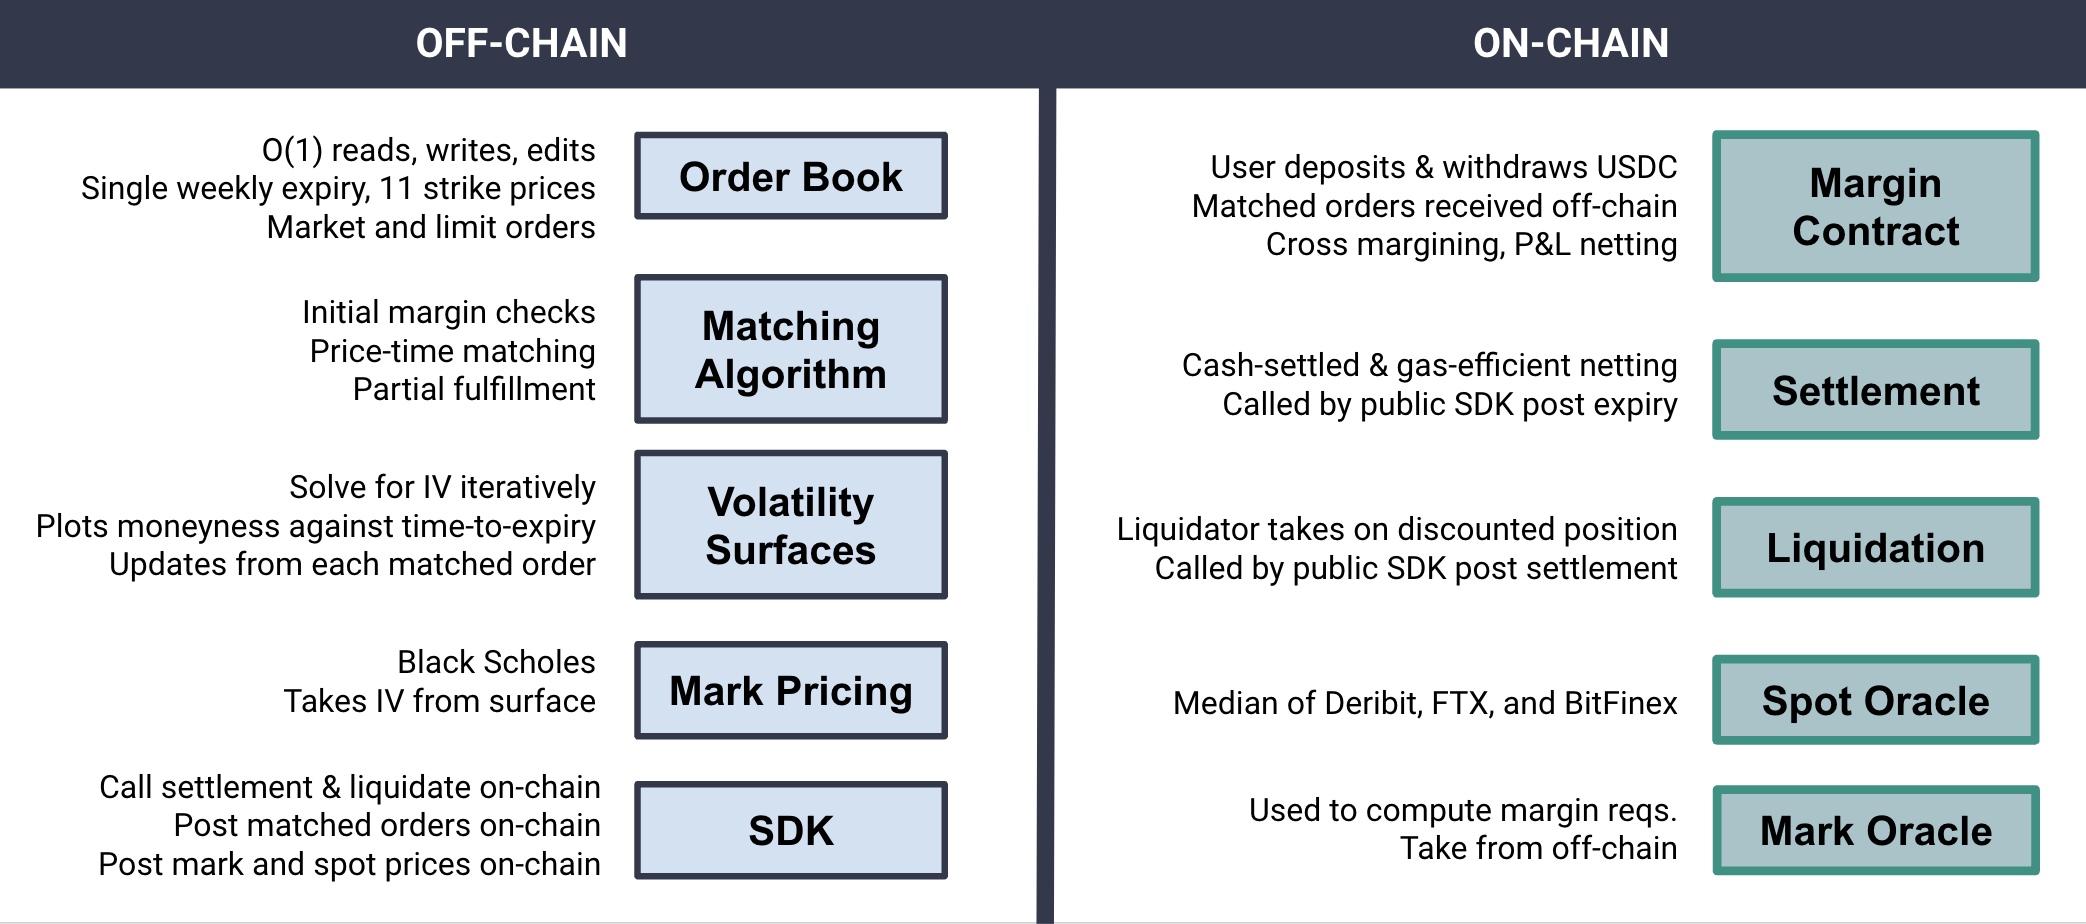
\includegraphics[width=0.9\textwidth]{images/overview2.png}
\caption{Our Order Book Architecture}
\end{figure}

\section{Background}

\noindent Order books are the dominant exchange structure in Traditional Finance. They allow market participants to express specific preferences for price and risk appetites, therefore enabling efficient price discovery. However, their first iterations did not translate as well to blockchain environments due to throughput constraints and issues when \href{https://angeris.github.io/papers/cfmm-ob.pdf}{blockchains experience outages} (e.g. Solana 2021). There is now heightened demand for cryptographically verified proof of funds, which centralized exchanges do not and can not offer. Furthermore, the increase in transaction throughput on Ethereum Layer 2s and the development of application-specific rollups as a service (e.g. \href{https://twitter.com/calderaxyz}{Caldera}) enables the order book hypothesis to be tested again in the Ethereum ecosystem. \\

\noindent As far as we know, there is no open source order book infrastructure apart from Serum on Solana. Our objective in the following paper is to make it easier for other builders to create order book based DeFi products. This paper follows our journey building an options order book and its important decision points. If you would like to discuss, please reach out to \href{https://twitter.com/WillMcTighe}{Will McTighe}. \\


\noindent Figure~\ref{fig:overview2} shows the off-chain and on-chain parts of the infrastructure. Our own conclusions led us to building the actual order book, order matching engine, mark pricing, and volatility surfaces off-chain. The on-chain components were settlement, liquidation and margin checks. As this is a working document, if you have any additions, please share them with us. \\

\subsection{Open-Source Code}

To complement this paper, we open-source code for both on-chain and off-chain components of our order book. We emphasize that although we did extensive testing ourselves, none of the code was deployed in practice nor audited. Please proceed with caution and at your own risk.
\begin{itemize}
    \item The server \url{https://github.com/pareto-xyz/pareto-orderbook-v1} is written in Golang, which was chosen for scalability and compatibility with existing ethereum SDKs. The code contains implementations for an order book, matching, and volatility surfaces for Black Scholes.
    \item The smart contracts \url{https://github.com/pareto-xyz/pareto-core-v1} are written in Solidity, and are responsible for maintaining matched orders, balances, and most importantly, process settlement and liquidation. A keeper plays an important role in maintenance.
    \item  The client \url{https://github.com/pareto-xyz/pareto-client-v1} is written in Python, and requires the user to supply their private key, similar to dydx's client. Generally, we aligned design choices with ones market makers are familiar with to reduce the integration time. This is often Python or C++. You may also want to make the client similar to Binance's given that is the dominant crypto exchange.
   \item Liquidation SDK \url{https://github.com/pareto-xyz/pareto-liquidation-sdk-v1} that allow users to track low margin accounts and perform liquidation. Liquidations will likely only be done by market makers given the convex risk exposure. They can alternatively be done off-chain using a Request For Quote (RFQ) system. More on this in Section \ref{sec:liquidation}.
   \item Oracle SDK \url{https://github.com/pareto-xyz/pareto-oracle-bot-v1} uploads pricing data, averaged over multiple sources, to smart contracts such that they are accessible on-chain. These are intended to be maintenance by the order book team.
   \item Frontend \url{https://github.com/pareto-xyz/pareto-app-v1} is written in React. This repository is incomplete in that it is not connected to the backend but serves as a starting point. 
\end{itemize}

\noindent We encourage readers to fork these repos and re-use them for their own purposes. This code will not be maintained but please reach out to \texttt{mike@paretolabs.xyz} with any technical questions.

\section{Order Book and Matching Algorithm}

In the following sections, we describe each of the components of an order book from Figure~\ref{fig:overview2} in more detail, providing empirical and technical annotations for design choices. To start, we focus on the book and matching algorithm, which are modeled after their TradFi counterparts.

\subsection{Order Book}

\noindent There are several important design choices when building an order book, but by far the most important is efficiency. It is of upmost importance to users that the order book is performant, especially during periods of high volatility.
Throughput requirements are very different for orders compared to matched trades: most orders are not matched. 
Order books need capacity to handle thousands of orders per second to support the creation, deletion, and editing of orders that market makers expect.
As one data point, each CEX market maker typically receives roughly 50 TPS to send, update and cancel their orders. As you will see \href{https://twitter.com/EliBenSasson/status/1458813552446345226/photo/1}{here}, DYDX-v3 normally only required 5-10 transactions per second (TPS) during the 2021 bull market but up to 35 TPS during volatility spikes. 
To this end, technical design choices optimize for speed. We have already discussed the choice of programming language in which compiled languages like C, C++, Java, and Go greatly outperform more user-friendly languages like Python. 
The next important decision point is to whether to build on-chain or off-chain.

\subsubsection{What are your options?}

We view three distinct options.

\begin{itemize}
    \item \textbf{On-chain Order Book \& Settlement on a General Purpose Chain} \quad Serum on Solana was the only example of this that we know of, though it may be possible on other high throughput chains (e.g. Aptos, Sui, etc.). This approach minimizes legal risks by maximising decentralization but should the chain become congested, the order book slows down and impacts user experience. Additionally, an on-chain order book would require a transaction fee per order placed, which is atypical of TradFi order books where placing an order is free. It is important to note that the market makers business model works when the cost of placing orders is basically zero and becomes much less sustainable if this cost rises even slightly.
    \item \textbf{Off-chain Order Book \& Settlement on a General Purpose Chain} \quad e.g. a DYDX-style order book on Arbitrum Nitro. We haven't seen an example of this tested in the wild yet. The benefit of this approach is you do not have to build or pay for application-specific roll up infrastructure. However, it is not clear that Ethereum L2 general purpose chains yet have sufficient throughput to support an order book. This approach also carries legal risks if you are unwilling to KYC users.
    \item \textbf{Off-chain Order Book \& Settlement on an Application-Specific Chain} \quad \href{https://twitter.com/dYdX}{DYDX}-V3 and \href{https://twitter.com/aevoxyz}{Aevo} are examples of this. The approach gives the protocol more control during periods of high volatility because transaction execution will not compete with other protocols. This approach carries some legal risks, particularly if you are a US-based entity. You could be classified as a US broker dealer and therefore have onerous KYC requirements. We are not lawyers but Miles Jenning at a16z wrote two helpful papers on decentralization considerations \href{https://a16zcrypto.com/wp-content/uploads/2022/06/dao-legal-framework-part-1.pdf}{here} and \href{https://a16zcrypto.com/wp-content/uploads/2022/06/dao-legal-framework-part-2.pdf}{here}.   
\end{itemize}

\subsubsection{Technical Considerations} 

\noindent In our implementation, it was important to ensure that adding, editing, and deleting orders were all O(1) operations. Further the order book needed to support different assets (e.g. BTC and ETH) as well as derivatives (e.g. options and futures). To accomplish this, the order book maintains a few data structures. It may be helpful to refer to the \href{https://github.com/pareto-xyz/pareto-orderbook-v1/tree/main/orderbook}{code} in reading below.
\begin{itemize}
    \item A map from a unique identifier to every order in the book. This enables constant-time look up once you know what order you are looking for. An order specifies a price and a quantity of an asset to buy or sell. 
    \item Orders were separated into asks (price a seller is willing to sell) and bids (price a buyer is willing to pay). Common queries will be for the lowest ask or highest bid.
    \item Asks (and also bids) are organized by strike and expiry such that orders for the same (strike, expiry) combo are stored together. 
    \item For a single (strike, expiry) combo, a red black tree is maintained to surface minimum and maximum prices. For each unique price, a linked list is maintained of order identifiers sorted by timestamp such that the earliest made order is held first.
    \item Separate order books are kept for different tokens and derivatives (e.g. calls and puts). 
\end{itemize}

\noindent With this design, a query for an ask or bid at a price for a derivative amounts to reading the head of a linked list, which is constant-time. Given a certain quantity to fulfill, one can keep reading from the head until the order is satisfied. All in all, our implementation reaches 200-300k transactions per second in timing tests. This may vary when deployed given bandwidth and network constraints. \\

\noindent In the chase for efficiency, it is inviting to parallelize the order book using multiple threads or workers. While this is indeed possible (and easy to do so in Go), we chose to refrain from it as parallelization introduces non-deterministic ordering. Sequential processing makes the book easier to manage and critically, easier to reproduce in the case of a temporary shutdown. 

\subsubsection{Order Types}

\noindent A sophisticated order book supports market orders,  limit orders, trigger orders, and potentially more but we chose to start with the bare minimum of market and limit orders. Market orders are fulfilled immediately by finding the best price at the desired quantity. Limit orders, when it is possible, are fulfilled immediately if the opposing side exists. If not, any unfulfilled quantity is added to the book. 

\subsubsection{Strike and Expiry Selection} 

In expiring derivatives, it is very important that you choose expiry dates and strike prices that are aligned with the largest pools of liquidity because it allows traders to hedge and trade your product elsewhere. For example, if you are building options products, check your strike prices and expiries are in-line with Deribit. Otherwise, you risk not taking advantage of existing liquidity as users are unable to precisely hedge your derivatives with instruments elsewhere. 

\subsection{Matching Algorithm} \\

The matching algorithm, as hinted by the technical design above, is a \textbf{price-time} matching algorithm with \textbf{partial fulfillment}. In particular, we use a FIFO, or first-in-first-out, heuristic. The algorithm is intuitively very simple: Find the unmatched order with the best price i.e. the lowest ask or the highest bid. In case that there are multiple unmatched orders, the order made at the earliest time is matched. Hence the term: "first in, first out". FIFO is typical but there are several alternatives described in detail \href{https://www.cmegroup.com/confluence/display/EPICSANDBOX/Supported+Matching+Algorithms}{here} that essentially either order only by price (e.g. pro rata) or auxiliary features. We chose FIFO given it is the most commonly found algorithm in practice. \\

\noindent Partial fulfillment is also simple and standard practice. In many cases, the quantities for buy and sell orders to be matched do not equal. In these cases, the matching algorithm performs partial fulfillment. For example, if there is a single buy order with quantity 100, and there are only SELL orders at quantities 50, 30, and 20, all three SELL orders will be matched to fulfill the larger BUY order. For a market buy order, the matched sell orders may be of different prices. For a market order, if any quantity is unable to be fulfilled, this is relayed to the user and the book is unchanged. For a limit order, any amount unable to be immediately filled (by an opposing limit order) is kept on the book. \\

\section{Settlement}

\noindent A key decision for any order book is the settlement asset. There are two options: \textbf{cash settled} (e.g. in USDC or an analogous stablecoin) and \textbf{physically settled} using the underlying asset (e.g. ETH, BTC). There are tradeoffs to either:
\begin{itemize}
    \item Often traders prefer cash-settled because it is easier to understand your risk profile. It is also less complex to cross-margin across different positions (e.g. ETH and BTC derivatives). Exchanges are more able to offer derivatives on long tail assets without exposing the exchange to additional risk of the underlying physical asset. For example, if someone sold PUT options on a shitcoin and used that token as collateral and the price went to zero, the seller's collateral would be worthless and they would owe a lot of money. If they could not pay it, the exchange would have to pay up with their insurance fund. This would not occur under cash settlement.
    \item Popular exchanges like Deribit are physically settled. Physically settled may be preferred by some investors who want to hold for the long term and sell upside in the meantime to earn yield.   
\end{itemize}

\noindent We chose cash-settled and believe there is space for more cash-settled DEXs.

\subsubsection{Technical Considerations} 
\label{sec:tech:settlement}

Settlement can be implemented efficiently on-chain as a map from addresses to an unsigned integer. Settlement in a regular interval (e.g. weekly or monthly) amounts to a single function call that loops through open matched trades (which are stored on-chain), computes profits and losses per position, and shifts balance from one entry to another in the map.
For a cash-settled order book, no actual token transfers are made (assuming no new deposits and withdrawals), making settlement cheap and efficient.
For a physically-settled order book, balances can still be stored as a map but additional logic must be made to swap a portion of the collateral held within the smart contract for the physical asset in case of a withdrawal. Due to this potential complexity, we opted for cash settlement.\\

\noindent In our design, there is a designated \textit{keeper} role who has permissions to call the settlement function.
Since we chose an off-chain order book and on-chain settlement, the keeper is also responsible for uploading matched trades: once a market or limit order is matched in the off-chain order book, the keeper must call a smart contract function to store the matched trade. For cost savings, this operation may be batched.
Once a ``round'' is over and settlement is complete, trades stored on-chain are deleted, resetting the contract for the next round. 
A separate smart contract should be deployed for different underlying assets and expiries. This can also be efficiently done through a factory contract. 

\subsection{Deposits and Withdrawals}

Deposits are relatively simple: a user can deposit at any time, which increases the user's balance stored on-chain immediately. This balance will serve as collateral for any new positions the user enters and determines what positions a user may participate in (see Section \ref{sec:marginframework}). 
We initially capped the amount of total balance a user can deposit into the smart contract. This is to prevent catastrophe losses in case of contract bugs. Over time, we expected to increase this cap, eventually removing it entirely.\\

\noindent Withdrawal is a more difficult operation, as allowing unlimited withdrawal can put users at risk of liquidation, especially if they have open positions. We defer to Section \ref{sec:accounthealth} for the exact formulas but emphasize that health checks (also called margin calls in derivatives literature) are necessary before withdrawal is permitted. However, unlike a vault, in which withdrawal is only allowed after a round is over, a user in an order book can theoretically withdraw assets from their balance at any point as long as it does not cause them to fail their health check. 

\section{Margin Framework}
\label{sec:marginframework}

\noindent A great margin framework is a balance between capital efficiency and risk management. The goal is to offer enough margin to make your exchange competitive with off-chain ones so users want to use it but does not blow up in Black Swan events (e.g. large price swings).
It only takes one black swan event to end an exchange. We have seen poor risk management lead to the collapse of other protocols (e.g. \href{https://cointelegraph.com/news/100m-drained-from-solana-defi-platform-mango-markets-token-plunges-52}{Mango Markets}). 
Despite this risk, it is also painfully apparent that capital inefficiency is why most options protocols to date have failed: on-chain equivalents offer far less leverage. Walking this fine line is one of the primary challenges in running an order book protocol. \\

\noindent The way to increase capital efficiency is through better margining and lower collateral requirements. The simplest and most inefficient approach is requiring users to put up \textit{100\%} of the collateral required to enter \textit{each} new position in the order book. The pro of this approach is that is inherits little to no risk for the user and the exchange. The obvious con is that the same amount of money can do more for the user elsewhere where collateral requirements are looser and risk is better understood.

\subsection{Types of Margin}
\label{sec:margintypes}

\noindent The main idea of margining is that not all positions are created equal. Some have opposite risk profiles. As a silly example, consider buying and selling the same asset in the order book. Without margining, a user may need to put collateral up for each of these positions. But since the two orders ``cancel each other out'', we may allow the user to enter both positions with far less collateral. \\

\noindent There are levels of sophistication to margining. We summmarize each below.

\begin{itemize}
    \item \textbf{Cross Position Margin} is when the collateral in a single margin account is shared across multiple positions. In an options order book, this could be across different positions in a single underlying (e.g. ETH) but different strikes or expiries, or across multiple underlyings (e.g. ETH and BTC), or both. Any excess margin from one position is automatically used to satisfy margin requirements for another position. Essentially, the margin is a shared pool.

    \item \textbf{Isolated Margin} reserves collateral for a single position. This \textit{isolates} its risk but means that this position can be liquidated even if you have excess collateral in your margin account. Often this is done by creating a separate account for a user and depositing their collateral in it. \textit{Why do this?} This is useful to isolate risky positions such that they do not bleed collateral from a margin account that other less risky positions rely on.
    
    \item \textbf{Position Netting} is simply netting off directional exposure in two positions of the same derivative. For example, if I buy and sell a call option with a \$1,500 strike price, this should net to leave no open positions and release your collateral. That is not the case in many derivatives protocols today. This can be combined with cross margining.
    
    \item \textbf{PnL Netting} is netting off directional exposure in two positions of different derivatives. This enables spread trades. See Zeta Markets' excellent \href{https://docs.zeta.markets/zeta-protocol/trading/options-contract-specifications/spread-accounts}{documentation}. You can view this as a generalization of position netting. Suppose you plotted the risk profile of each position then summed across all positions: the resulting risk is used to determine collateral requirements rather than summing the requirements of each position independently. This can be combined with cross margining.
    
    \item \textbf{Portfolio Margin} is a risk-based margining system that takes a portfolio of positions and does sensitivity analysis with price and volatility shocks to determine the amount of collateral required. In TradFi, only professionals and market makers have access to this. There are several frameworks for this including FINRA and CME SPAN.
\end{itemize}

\noindent Based on our market research and the time required to build each of these well, we prioritized in the following order: 1. Cross-position margin, 2. Position Netting, 3. PnL Netting, 4. Isolated Margin and 5. Portfolio Margin. Portfolio margin is important for market makers but meaningfully more complex and can lead to big losses if not carefully implemented and maintained. 
As an MVP, we recommend starting with just cross-position margin and position netting, which we believe to already be an improvement to the status quo without taking on too much risk. 

\subsubsection{Application: Delta Hedging} 

\noindent Margining gives the ability to get \textit{credit} for having positions that offset each other. This is not particularly easy in the current state of DeFi. With cross margining and netting, credit could be shared across different instruments (e.g. spot, expiring futures, perpetuals, options) in the same underlying asset. For example, if you are long 1 ETH and short 1 ETH perpetual you are delta hedged, that is, you are not meaningfully exposed to changes in the underlying price of ETH. Many protocols require you to post collateral for both which is strictly less capital efficient.


\subsection{Collateral Requirements}
\label{sec:collateralreqs}

\noindent The next important question is \textit{How much collateral should you require users to deposit?} There are several well-known frameworks to think about this: 

\begin{itemize}
    \item \href{https://en.wikipedia.org/wiki/Regulation_T}{Reg T} is a set of heuristics or guidelines that are case-by-case depending on the derivatives. See \href{http://www.themargininvestor.com/option-strategies---reg-t-margin.html}{here} for an example in TradFi options. The requirements of RegT are quite conservative and err towards covering 100\% or a large fraction of the potential losses with collateral. 
    \item \href{https://www.cmegroup.com/clearing/risk-management/span-overview.html}{CME SPAN} is also a form of portfolio margin. It enables a lot of leverage and is not sufficient out of the box because it exposes exchanges to too much risk. Hard to do on-chain because it is dynamic. It sums the positions in an account and simulates price shocks and uses that to determine margin requirements. It does not include volatility shocks.
    \item \href{https://www.finra.org/rules-guidance/key-topics/margin-accounts}{FINRA} is a form of portfolio margin. It is slightly more conservative than CME SPAN in that it includes some volatility shocks, rather than just price shocks. However, still needs some tweaks. You should not think of these tools as sufficient out-of-the-box. 
\end{itemize}

\noindent You can also look at the margin requirements of successful exchanges that have stood the test of time for inspiration (e.g. Binance, Deribit). To state the obvious, it is safer to start more conservatively by requiring more margin (e.g. RegT) and offering lower volatility assets (e.g. starting with BTC, ETH) and become more adventurous as your risk framework performs in the wild. The more illiquid the market, the more easily it can be manipulated. In options, selling options has more risk than buying options, so requires a larger proportion of the underlying as collateral. Sophisticated exchanges generally have in-house portfolio margining systems that have been tweaked from experience. 

\subsection{Margin Checks}
\label{sec:accounthealth}

The purpose of margining is to determine a threshold: if a user's deposited collateral is less than this threshold, then their position is deemed ``risky'' and can be liquidated to prevent potential larger losses. 
The margin account is where all of a user's collateral is stored (In Section~\ref{sec:tech:settlement}, we described this as a map in a smart contract). Margin checks are constantly being performed by an order book. What a user is allowed to do depends on them passing a specific margin check. To ensure users' do not take on too much risk, margin checks are completed when users:
\begin{itemize}
    \item Create, edit, or delete new orders
    \item Enter new positions (i.e. when orders get matched)
    \item Deposit funds
    \item Withdraw funds
\end{itemize}

\noindent A margin check computes the following expression:

\begin{equation}
    \textup{Balance} + \textup{uPnL} > \textup{IM}(\textup{open orders}) + \textup{MM}(\textup{open positions})
    \label{eq:margincheck}
\end{equation} 

\noindent What does this equation mean?
\begin{itemize}
    \item \textbf{Balance} is the amount of USDC (cash) held within the user's margin account (i.e. in the smart contract). This is the amount the user deposited plus any realized PnL (profit) from previous positions that have not been withdrawn.
    \item \textbf{Unrealized PnL (uPnL)} is the profit and losses from all open positions. It is calculated with the current spot price and changes as price changes. Depending on your risk tolerance you can play with this term. For example, to be conservative, if the sum is greater than zero, you can set this to zero until profits are realized i.e. $min(\textup{uPnL}, 0)$. 
    \item \textbf{Open Positions}: live positions that have already been matched with a counterparty. Above, we also referred to this as ``matched trades''.
    \item \textbf{Open Orders}: a user's open orders that are in the order book. They are not matched positions but can become matched if a counterparty matches with them. For retail users it is common to require that they have sufficient collateral in their margin account for each open order.
    \item \textbf{Initial Margin (IM)} is a function that specifies the margin required for all open  orders. It is not used for matched orders. IM is typically higher than MM, meaning it is more expensive to open an order than stay in one. This also provides users a liquidation buffer. 
    \item \textbf{Maintenance Margin (MM)}: Required margin on open positions. This value fluctuates over the lifetime of a position given changes to spot price and the user's balance as well as unrealized P&L (e.g. user enters more positions). 
\end{itemize}

\noindent In practice, you compute variations of this inequality depending on the user's actions. For example, when withdrawing, you may only check maintenance margin if you wish to be less conservative. For explanatory purposes, the formula above tends to be most clear. The terms on the left hand side represent the user's assets, whereas the terms on the right represent the user's liabilities. This is similar to a ``health check'' from popular DeFi lending protocols like \href{https://docs.euler.finance/getting-started/white-paper#liquidations}{Euler} and \href{https://docs.angle.money/angle-borrowing-module/vaults/liquidations}{Angle}. 
  
\subsubsection{Technical Considerations}

In a design where the order book is entirely on-chain or entirely off-chain, computing margin checks is straightforward once you decide the margining system. In a design with on-chain and off-chain components, proper margin checks require communication between the two components. In our design, the smart contract has no knowledge of open orders; it only knows open positions. Similarly, the off-chain order book only knows open orders and stops tracking once they are matched. 
When performing a margin check from the off-chain order book, a smart contract is required to fetch a user's maintenance margin. When performing a margin check from the smart contract, you have two options: (1) you can ignore the initial margin entirely or (2) you can broadcast initial margin requirements to an oracle contract. We opted for (1) for its simplicity though (2) is less risky.

\subsubsection{Case Study: Margin Check with RegT for Options}

We give an example of our exact margin requirements. Note that this is specific to options. These heuristics have not been tested in practice, but could serve as a starting point.

\begin{table}[h!]
    \centering
    \begin{tabular}{c|c|c}
         \textbf{Option} & \textbf{Side} & \textbf{IM} \\
         \hline
         Call & Long & $\min\left(\textup{mark}, \textup{10\% of spot}\right)$ \\ 
         Call & Short & $\max\left(\textup{20\% of spot - OTM amount}, \textup{12.5\% of spot}\right)$  \\
         Put & Long & $\min\left(\textup{mark}, \textup{10\% of spot}\right)$ \\ 
         Put & Short & $\min\left( \max\left( \textup{20\% of spot - OTM amount}, \textup{12.5\% of Spot} \right), \textup{50\% of strike} \right)$ \\ 
    \end{tabular}
    \caption{Initial margin requirements}
    \label{tab:my_label}
\end{table}

\begin{table}[h!]
    \centering
    \begin{tabular}{c|c|c}
         \textbf{Option} & \textbf{Side} & \textbf{MM} \\
         \hline
         Call & Long & $\min\left(\textup{mark}, \textup{6.5\% of spot}\right)$ \\ 
         Call & Short & $\max\left(\textup{10\% of spot - OTM amount}, \textup{8\% of spot}\right)$  \\
         Put & Long & $\min\left(\textup{mark}, \textup{6.5\% of Spot}\right)$ \\ 
         Put & Short & $\min\left( \max\left( \textup{10\% of spot - OTM amount}, \textup{8\% of spot} \right), \textup{50\% of strike} \right)$ \\ 
    \end{tabular}
    \caption{Maintenance margin requirements}
    \label{tab:my_label}
\end{table}

\noindent In the tables above, the ``OTM amount'' represents the amount that the spot is ``out-the-money''. For calls, this is computed as $\max\left(\textup{strike} - \textup{spot}, 0 \right)$. For puts, it is the opposite $\max\left(\textup{spot} - \textup{strike}, 0 \right)$. The ``strike`` price is set by the option; the ``spot'' price is obtained from an oracle (see Section~\ref{sec:oracles}); the ``mark'' price is computed as in Section~\ref{sec:mark} using Black-Scholes.

\subsection{Mark Pricing}
\label{sec:mark}

This section is specific to options but likely still useful for a broader class of derivatives. The case study hinted towards the importance of mark pricing in setting margin requirements. The goal of mark pricing is to prescribe the value of an options contract such that we can quantitatively evaluate the returns and risk of a position. This is typically done using Black-Scholes:
\begin{align}
\textup{Call price} &= \textup{spot} * \textup{CDF}(d_1) - \textup{strike} * e^{-\textup{rate} * \textup{time to expiry}} * \textup{CDF}(d_2) \\
\textup{Put price} &= \textup{strike} * e^{-\textup{rate} * \textup{time to expiry}} * \textup{CDF}(-d_2) - \textup{spot} * \textup{CDF}(-d_1)
\end{align}

\noindent In particular, the price changes as a function of the spot price and the time left before the option contract expires. Generally, the value of an option is greater with more time til expiry since there is room for the price to move in-the-money. The term ``CDF'' represents the cumulative distribution function for a standard Gaussian distribution. Further, the variables $d_1$ and $d_2$ are defined as:
\begin{align}
    d_1 &= \frac{\log\left(\frac{\textup{spot}}{\textup{strike}}\right) + \textup{time to expiry} + \left(\textup{rate} + \frac{\textup{iv}^2}{2}\right)}{\textup{iv} * \sqrt{\textup{time to expiry}}} \\
    d_2 &= d_1 - \textup{iv} * \sqrt{\textup{time to expiry}}
\end{align}

\noindent The variable ``rate'' represents a risk-free rate, which we set to the lending APR using Compound.  For the purposes of setting margin requirements, exchanges with deep liquidity may replace mark pricing with average of the highest bid and lowest ask. 

\subsubsection{Implied Volatility} 
\label{sec:bisection}

One of the necessary components for mark pricing is implied volatility (``iv''), which is not known a-priori. But, since we have the option price for every matched order we can attempt to back-solve for implied volatility using the Black Scholes formula.\\

\noindent Since there is no closed form solution for implied volatility from call/put price, we resort to a reliable iterative approach: the bisection method. Assume a minimum and maximum implied volatility e.g. minimum of 0 and maximum of 10 (1000\%). Choose an error tolerance e.g. 1e-4 and a maximum number of iterations e.g. 10000. Consider the following algorithm (written in Python for easy reading):

\begin{figure}[h]
    \centering
    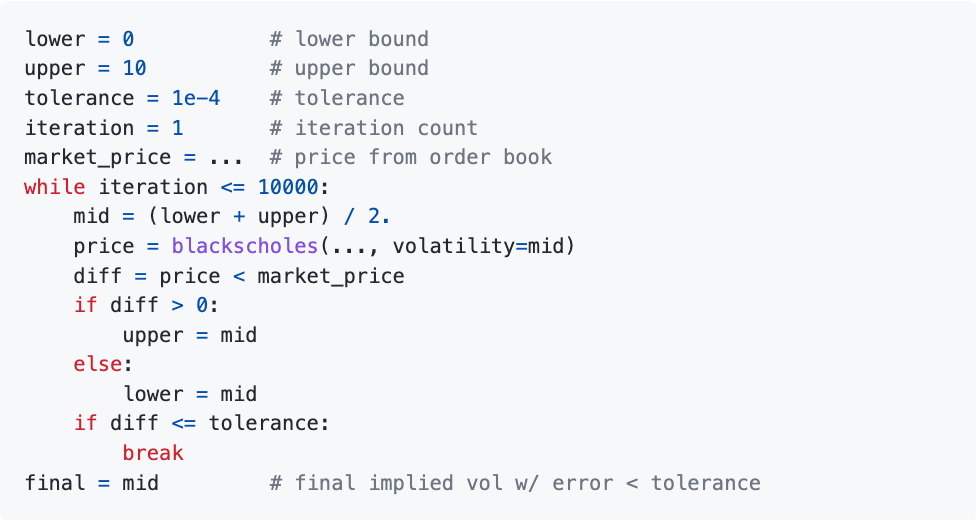
\includegraphics[width=0.8\textwidth]{images/code.png}
\end{figure}

\noindent The convergence of the algorithm is fast and can efficiently be performed off-chain. 

\subsubsection{Volatility Surfaces} 
\label{sec:surfaces}

While Section~\ref{sec:bisection} provides a solution, we know that it is flawed. One of the core assumptions of the Black Scholes model is constant volatility, and empirical evidence shows this is not true. In practice, the implied volatility rises further out-the-money or int-the-money compared to at-the-money. If we plot the volatility as a function of the strike, we build a ``U''-like shape resembling a \href{https://en.wikipedia.org/wiki/Volatility_smile}{smile}. In fact, as time creeps towards the expiry, the implied volatility tends to increase as well. Given that now we know volatility is not constant in two dimensions, a single number is not sufficient.\\

\begin{figure}[h]
\centering
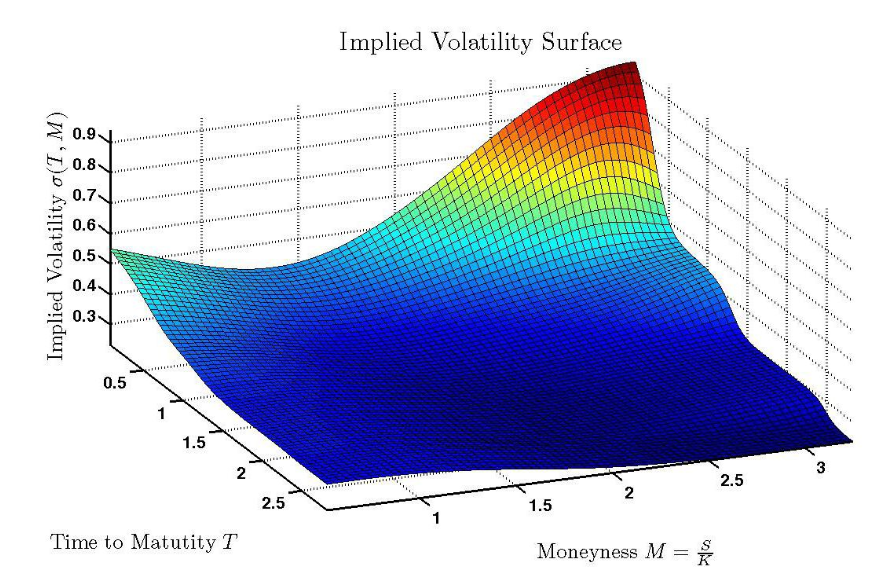
\includegraphics[width=0.5\textwidth]{images/slope.png}
\end{figure}

\noindent Our approach is to build our own ``volatility surface'', which tracks implied volatility over time and ``moneyness'' (spot divided strike price) axes. At the start, we initialize the surface to a ``guess'' for IV. For each new matched order, we use the market price to backsolve for implied volatility. The matched order also contains a spot, strike, and time-to-expiry. We find the closest point on the volatility surface. Suppose this is at index $(i, j)$; then, we update the point using a weighted sum
\begin{equation}
    \textup{surface}[i][j] = w * \textup{surface}[i][j] + (1-w) * \textup{IV from Black-Scholes}
\end{equation}
where $w$ decides how much to emphasize new data. Optionally, we may update points nearby index $(i,j)$ as well to ``smooth'' the surface. For unmatched orders, the surface is not updated. The surface is also not reset once an option expires; it will continue to the next round. \\

\noindent We can query for a new option's IV by finding the closest $N$ moneyness ticks $(m_1, \ldots, m_N)$ and closest two time to expiries $(t_1, \ldots, t_N)$ on the surface.  Using the $N^2$ points $(m_1, t_1), (m_1, t_2), \ldots$, we can look up the IV at each point and average them to a final estimate. \\

\noindent There is a choice between building the surface on-chain or off-chain:

\begin{itemize}
    \item \textbf{Transparent} $\quad$ The benefit of building the surface on-chain is less communication off-chain. The smart contract could be ``self-contained'' which is less prone to hacks and bugs.
    \item \textbf{Low Resolution} $\quad$ The challenge of building on-chain volatility surfaces is resolution. Off-chain, we can divy the moneyness and time-to-expiry axes into as many discrete points as we would like, building a fine-grained surface. On-chain, we need to limit ourselves to a small set of discrete points e.g. 20 per axes for a total of 400 points. The tradeoff of storage cost and resolution may result is less trustworthy implied volatility estimates.
    \item \textbf{Off-chain Sources} $\quad$ A strength of the off-chain volatility surface is the ability to incorporate other data sources. One of the fundamental flaws of estimating IV using only your exchange is that likely a significant portion of trading volume happens outside of your order book. Since IV only updates when orders are matched in your book, the surface will lag behind. For a new order book, this can be quite problematic. We recommend implementing an IV backstop using a large exchange like Deribit, or ideally multiple other exchanges. When our IV surface is more than 2\% different than Deribit's IV, we can update our surface with Deribit's value.
\end{itemize}

\noindent Weighing these benefits and consequences, we chose to store the volatility surface off-chain, primary due to (3). Broadcasting our mark prices on-chain is done through oracles, as in Section~\ref{sec:oracles}.
 
\section{Liquidation Engine}
\label{sec:liquidation}

\textbf{Disclaimer: Liquidation is the part we spent the least amount of time on.}

\subsection{Liquidations}

\noindent Liquidations are important to ensure the exchange remains solvent. Liquidations begin when a margin account fails a margin check as defined in Section~\ref{sec:accounthealth}. If Equation~\ref{eq:margincheck} no longer holds; that is, a user's liabilities exceed their assets, they are liable for liquidation.\\

\noindent Liquidations can take place \textbf{on-chain} or \textbf{off-chain}. As always, there are trade offs:
\begin{itemize}
    \item \textbf{On-Chain Liquidation} is a permissionless liquidation process that can be initiated by any EOA. An EOA will conduct a margin check on another account via a smart contract call and if the account fails the margin check, its positions can be liquidated. The trade off is that if this happens to slowly due to network congestion, losses on your exchange can get very large. Often, market makers will run liquidation bots as they are sophisticated enough to manage the associated risks. 
    \item \textbf{Off-Chain Liquidation} could involve doing liquidations RFQ style to market makers who can hedge their exposure either on your exchange or elsewhere. While this can be quite profitable for market makers, the trade off is that it is obviously not permissionless.
    
\end{itemize}


\subsubsection{What Happens Upon Liquidation?}

This section assumes an options order book. Suppose a user's position is successfully liquidated. Then, the liquidator effectively purchases the position at the mark price of the option. The liquidator assumes the role of the original user. For example, if a user sold a call and was liquidated, the liquidator is now the seller of the call. The buyer of the call is unaffected by the liquidation and retains the same position.\\

\noindent There are additional considerations to also bear in mind:
\begin{itemize}
    \item \textbf{Partial liquidations} $\quad$ Customers prefer if you liquidate position-by-position rather than a whole account. Consider starting with the most toxic positions. We opted to start with short positions sorted by the uPnL. Positions with positive payoff cannot be liquidated. Positions that if liquidated, results in higher margin requirements (e.g. a short position that is cross margined or netted with a long position) cannot be liquidated. A margin check is made after every liquidation. If the margin account is no longer below margin, no further positions can be liquidated. Conversely, liquidators can liquidate one or more of the positions and leave the user still below margin (though less than before). There are a lot of edge cases, and this code should be carefully tested. 
    \item \textbf{Liquidation discounts} $\quad$ On their own, it may not be profitable to liquidate a position as to incentivize liquidators. Ideally the incentives to liquidate an account increase as their account health score decreases (see \href{https://docs.euler.finance/getting-started/white-paper#liquidations}{Euler} and \href{https://docs.angle.money/angle-borrowing-module/vaults/liquidations}{Angle}). We chose that a portion of the maintenance margin held by the user for the liquidated position is re-distributed: we chose to allocate 25\% to be transferred to the liquidator's margin account whereas 10\% is transferred to the insurance fund (see Section~\ref{sec:insurance}). The liquidator must pass the same margin check above after taking on the new position. If they do not, all changes will reverted. The margin check is performed prior to the reward. That is, liquidators cannot rely on the liquidation fee to pass the margin check.
\end{itemize}

\noindent It is important to emphasize to liquidators that liquidation is not risk-free. The inherited position can sour, even taking any incentives given into account. 

\subsection{Insurance Fund}
\label{sec:insurance}

\noindent If your liquidation process fails, then toxic unfunded positions remain on an exchange. Typically, exchanges have an insurance fund to make counterparties whole. It is market practice to make counterparties completely whole. Insurance funds are often funded with transaction and liquidation fees. \\

\noindent There is an interesting question on what to do once your insurance fund runs out. We have seen a couple of approaches:
\begin{itemize}
    \item \textbf{Socialized Losses} is a common approach where all accounts proportionally share the losses based on some metric, like their deposited collateral or profit amount. This approach is considered \textit{fair} but could potentially set off a liquidation cascade where socialized losses cause users who previously passed the margin check to now fail.
    \item \textbf{Deleveraging} is an approach used by DYDX. It involves offsetting negative-balance accounts with the profits from highly leveraged accounts. This reduces the amount of leverage in the system and will not set off a liquidation cascade but punishes the most profitable (and risk taking) and so could be construed as \textit{unfair}.
\end{itemize}

\section{Oracles}
\label{sec:oracles}

\noindent If you have off-chain infrastructure, oracles as the medium to communicate between the off-chain infrastructure and on-chain smart contracts. Keeping oracle data feeds up-to-date is costly but very important. Oracle feeds were to be updated at the earlier of every 30 seconds or a 1\% price change in the underlying asset. Bear in mind, this could be way too slow. 

\subsection{Spot Oracles}

\noindent Spot prices are required for mark pricing as well as computing margin requirements. The main considerations that effect your design choice are price manipulation, which could result in toxic flow and liquidations. Our options were creating an oracle of CEX prices, Chainlink or AMM Oracles. \\

\begin{itemize}
    \item \textbf{Chainlink} $\quad$ We did not use Chainlink because to our knowledge, Chainlink prices update in discrete jumps of ~2\% price changes in underlying assets. In leveraged instruments like options with convex payoffs, waiting for a 2\% jump is too large. We had also heard of instances when Chainlink's oracles being paused resulting in \href{https://blog.venus.io/venus-protocol-official-statement-regarding-luna-6eb45c3cb058}{hacks}. 
    \item \textbf{AMMs} $\quad$  An alternative approach would be to use the Uniswap price for a given pool. This price feed is continuous but exposes some MEV and price manipulation risk, particularly for less liquid assets. One attack vector opened up with Ethereum's shift to Proof of Stake. \textit{Why?} Because Proof of Stake validators know ahead of time when they are going to validate a block. So on block $n-1$ they can manipulate a price, and know with certainty that on block they can arbitrage themselves back. Sometimes block validators will get two blocks in a row. It is quite a hard thing to pull off and requires a lot of capital but should be noted as a risk. 
    \item \textbf{Centralized Exchanges} $\quad$  Our approach involved building our own oracles by taking the median asset price from Binance, FTX (RIP) and BitFinex's APIs. Using prices from multiple exchanges with deep liquidity reduces the risk of price manipulation. This median price was to be posted on-chain as an oracle contract, updating at least every 30 seconds.
\end{itemize}

\subsection{Risk-free Rate Oracle}

For options pricing, the risk-free interest rate is required. In TradFi this is often the US government bond yield but there is not consensus on what this should be in Web3. 
\begin{itemize}
    \item \textbf{Lending Rate} $\quad$ \href{https://insights.deribit.com/industry/option-quotes-using-forwards/}{Greg Magadini} argued for stablecoin lending rates and we initially went with the APR from supplying USDC to Compound v2, which can be obtained from their API. This rate was to be posted on-chain as an oracle contract, updating at least every 30 seconds.
    \item  \textbf{Expiring Futures} Another approach, taken by \href{https://docs.zeta.markets/zeta-protocol/zeta-infrastructure/margin-system/mark-pricing}{Zeta Markets} on Solana is to price options based on expiring futures, which have an implied risk-free rate (computed  by backsolving). This has the benefit of letting the free market define this variable but could be problematic in a low liquidity environment when pricing may be stale.
\end{itemize}
Generally, the risk-free rate has less impact on mark pricing than spot price. The rate is also less likely to fluctuate wildly. As such, this oracle should be cheaper and easier to maintain.

\subsection{Mark Price Oracles} 

Using volatility surfaces as constructed in Section~\ref{sec:surfaces}, we compute mark price for each instrument in our order books and post these values in an oracle contract. Given their large impact on margining and hence liquidations, these are updated at the same interval as spot price oracles. 

\section{Miscellaneous Considerations}

Considerations for working with market makers:
\begin{itemize}
    \item \textbf{Integrate with Fireblocks} $\quad$ If you want professional market makers to fill your order book, then know that many custody their assets with Fireblocks. If you only use Metamask, they are less encouraged to add volume on your exchange. 
    \item \textbf{Handling Bursts} $\quad$ Often an order book has API rate limits but market makers update their order book pricing in bursts (e.g. use 1 minute's worth of API calls in 6 seconds). This is something you will need to accommodate at scale. One of the benefits of off-chain order books is that supporting burst API calls is much easier. 
    \item \textbf{Co-location} $\quad$ This only applies if your order book is off-chain. It reduces the latency for market makers and makes them happier. It entails having your order book running on a server that is co-located (i.e. plugged into) their servers. This is likely more useful for a more mature product. For instance, Deribit offers this. 
    \item \textbf{No Initial Margin Checks} $\quad$ For market makers, it will be very capital inefficient for them to have capital reserved for all their open orders, so they will want margin checks just before orders are matched.
\end{itemize}

\noindent Considerations for your front end:
\begin{itemize}
    \item \textbf{Separate frontends} $\quad$ An order book product may be serving two very different user groups: retail and sophisticated traders. Consider separate frontends: one to enable retail traders to easily understand and interact with the order book, and one to enable sophisticated traders to take on complex positions to achieve a specific risk profile. 
\end{itemize}

\noindent Considerations for options products:
\begin{itemize}
    \item \textbf{Delta hedging} $\quad$ A popular strategy in TradFi is delta-hedging options positions with futures to reduce risk associated with price movement in the underlying asset (e.g. ETH). In crypto, there may be interesting variations of this: (1) offering a futures book along with an options book; (2) aligning with an existing futures book; (3) incorporating perps (non-expiring futures).
\end{itemize}

\section{Order Book Business Ideas}

We conclude with two more practical applications of a crypto order book. 

\subsubsection{Idea 1: AMM as a Market Maker in an Order Book}
\noindent People often characterize order books as competing with AMMs. However, we believe there is a world where they can work together in which an AMM acts as a market maker on an order book. In this scenario, the AMM consolidates liquidity and allows retail users to offer pricing to traders, whilst professional market makers can offer pricing directly into the order book. This also reduces the order book's dependence on professional market makers, encouraging decentralization.

\subsubsection{Idea 2: Off-Chain Order Book with On-Chain Settlement to Compete with CEXs} 
\noindent The key issue in recent crashes (e.g. 3AC, FTX) has been centralized entities being dishonest about their assets and leverage. Nevertheless, centralized exchange users also care about the performant features of a traditional CEX. A simple idea to address both of these concerns would be to build an exchange with only one decentralized component, settlement and asset storage, providing cryptographic proof of assets. Anyone could query the smart contract to view their balance and know that it must be correct. It could even do KYC on users and register with the relevant US regulatory entities. Additionally, building on StarkEx would also enable private transactions. 

\section{Acknowledgements}

We stood on the shoulders of giants to write this. Many of our insights came from fruitful conversations with practitioners in the field. A special thanks goes to Chris Grace, Ryan Grace, and Hao Yang for their guidance and expertise, as well as the Zeta markets team, who pioneered an on-chain options order book and many market makers kindly shared the important considerations for them.

\end{document}